\appendix
\section{Simulation-based Quantum Volume Estimation for Si/SiGe (Campaign Appendix)}\label{app:qv-campaign}

This appendix documents how simulated Quantum Volume (QV) was estimated from literature-derived device parameters and summarizes the results of a small Latin Hypercube Sampling (LHS) campaign. The goal is to show, in a controlled simulation setting, how realistic ranges of single- and two-qubit fidelities, coherence times, crosstalk, and SPAM parameters translate into IBM-style QV outcomes.

\subsection{Methodology and decision rule}
We follow the IBM Quantum Volume protocol for width $m$ (and equal depth $m$):
\begin{enumerate}
    \item For each width $m$, generate $N=100$ random square circuits following the QV prescription and transpile/schedule subject to nearest-neighbor constraints.
    \item For each circuit, compute the heavy-output probability (HOP) by first obtaining the ideal (noiseless) output probabilities and identifying ``heavy'' bitstrings with probability above the median; then run a noisy simulation with $5{,}000$ shots and estimate the observed heavy-output frequency.
    \item Aggregate across the $N$ circuits to obtain a sample mean HOP and a 95\% bootstrap confidence interval $[\mathrm{CI}_\mathrm{low},\,\mathrm{CI}_\mathrm{high}]$.
    \item Pass criterion (per IBM): declare width $m$ as passed if both the sample mean and the lower 95\% CI bound exceed $2/3$.
\end{enumerate}
The achieved Quantum Volume is then defined as $\mathrm{QV} = 2^{m^*}$ for the largest width $m^*$ that passes. Because finite-sample statistics can introduce mild non-monotonicity (e.g., an occasional pass at $m{+}1$ when $m$ narrowly fails), we report the maximum passing width observed and indicate any such occurrences explicitly.

\subsection{Noise model construction from literature parameters}
Device parameters were sampled via LHS from ranges compiled from recent Si/SiGe spin-qubit literature (see main text and \texttt{campaign\_manifest.json}). The simulator constructs a composite noise model with coherent and stochastic components using the following mappings:
\begin{itemize}
    \item Average fidelity to depolarizing probability:
    \[
      p_{1\mathrm{Q}} = 2\,(1 - F_1),\qquad p_{2\mathrm{Q}} = \tfrac{4}{3}\,(1 - F_2).
    \]
    \item Amplitude and phase damping during a gate of duration $\tau$:
    \[
      p_\mathrm{amp} = 1 - e^{-\tau/T_1},\qquad p_\phi = 1 - e^{-\tau/T_\phi},\quad \text{with } \tfrac{1}{T_\phi} = \tfrac{1}{T_2} - \tfrac{1}{2T_1}.
    \]
    \item Quasi-static detuning to model slow drift via $T_2^*$:
    \[
      \Delta \sim \mathcal{N}\!\bigl(0,\,\sigma^2\bigr),\quad \sigma = \tfrac{\sqrt{2}}{T_2^*},
    \]
    sampled once per circuit.
\end{itemize}
SPAM, control crosstalk, and residual ZZ coupling are included per-sample using the values in each YAML configuration; two-qubit gate time is fixed at 40\,ns; single-qubit gate times are sampled in the 60--70\,ns range.

\subsection{Campaign setup}
The campaign evaluated $5$ configurations (\texttt{lhs\_sample\_0000} through \texttt{0004}) drawn by LHS over the ranges listed in the manifest (e.g., $F_2\in[0.92,\,0.9981]$, $T_2\in[245\,\mathrm{ns},\,3.1\,\mathrm{ms}]$, $T_2^*\in[0.36,\,20]$\,$\mu$s, control crosstalk $\in[0.44\%,\,1.85\%]$). Each configuration simulated widths $m=2,\dots,12$ with $N=100$ circuits per width and $5{,}000$ shots per circuit.

\subsection{Results summary}
Table~\ref{tab:qv-summary} summarizes the simulated QV outcomes. The maximum passing width $m^*$ and corresponding QV are reported, together with the first failing width when applicable.

\begin{table}[!htb]
  \centering
  \caption{Simulated QV outcomes by LHS configuration (pass threshold $2/3$ with 95\% CI).}
  \label{tab:qv-summary}
  \begin{tabular}{lcccc}
    \hline
    Configuration & Max pass $m^*$ & QV $=2^{m^*}$ & First fail width & Notes \\
    \hline
    lhs\_sample\_0000 & 5 & 32 & 6 & Monotonic (2--5 pass, 6+ fail) \\
    lhs\_sample\_0001 & 7 & 128 & 6 & 6 fails on CI, 7 passes (finite-sample non-monotonic) \\
    lhs\_sample\_0002 & 11 & 2048 & 12 & Strong, passes 2--11, 12 fails (mean and CI) \\
    lhs\_sample\_0003 & 5 & 32 & 6 & Monotonic (2--5 pass, 6+ fail) \\
    lhs\_sample\_0004 & 5 & 32 & 6 & Monotonic (2--5 pass, 6+ fail) \\
    \hline
  \end{tabular}
\end{table}

Figure~\ref{fig:qv-overview} illustrates the campaign-wide comparison, and Figure~\ref{fig:qv-waterfall} shows the pass/fail transitions by width.

\begin{figure}[!htb]
  \centering
  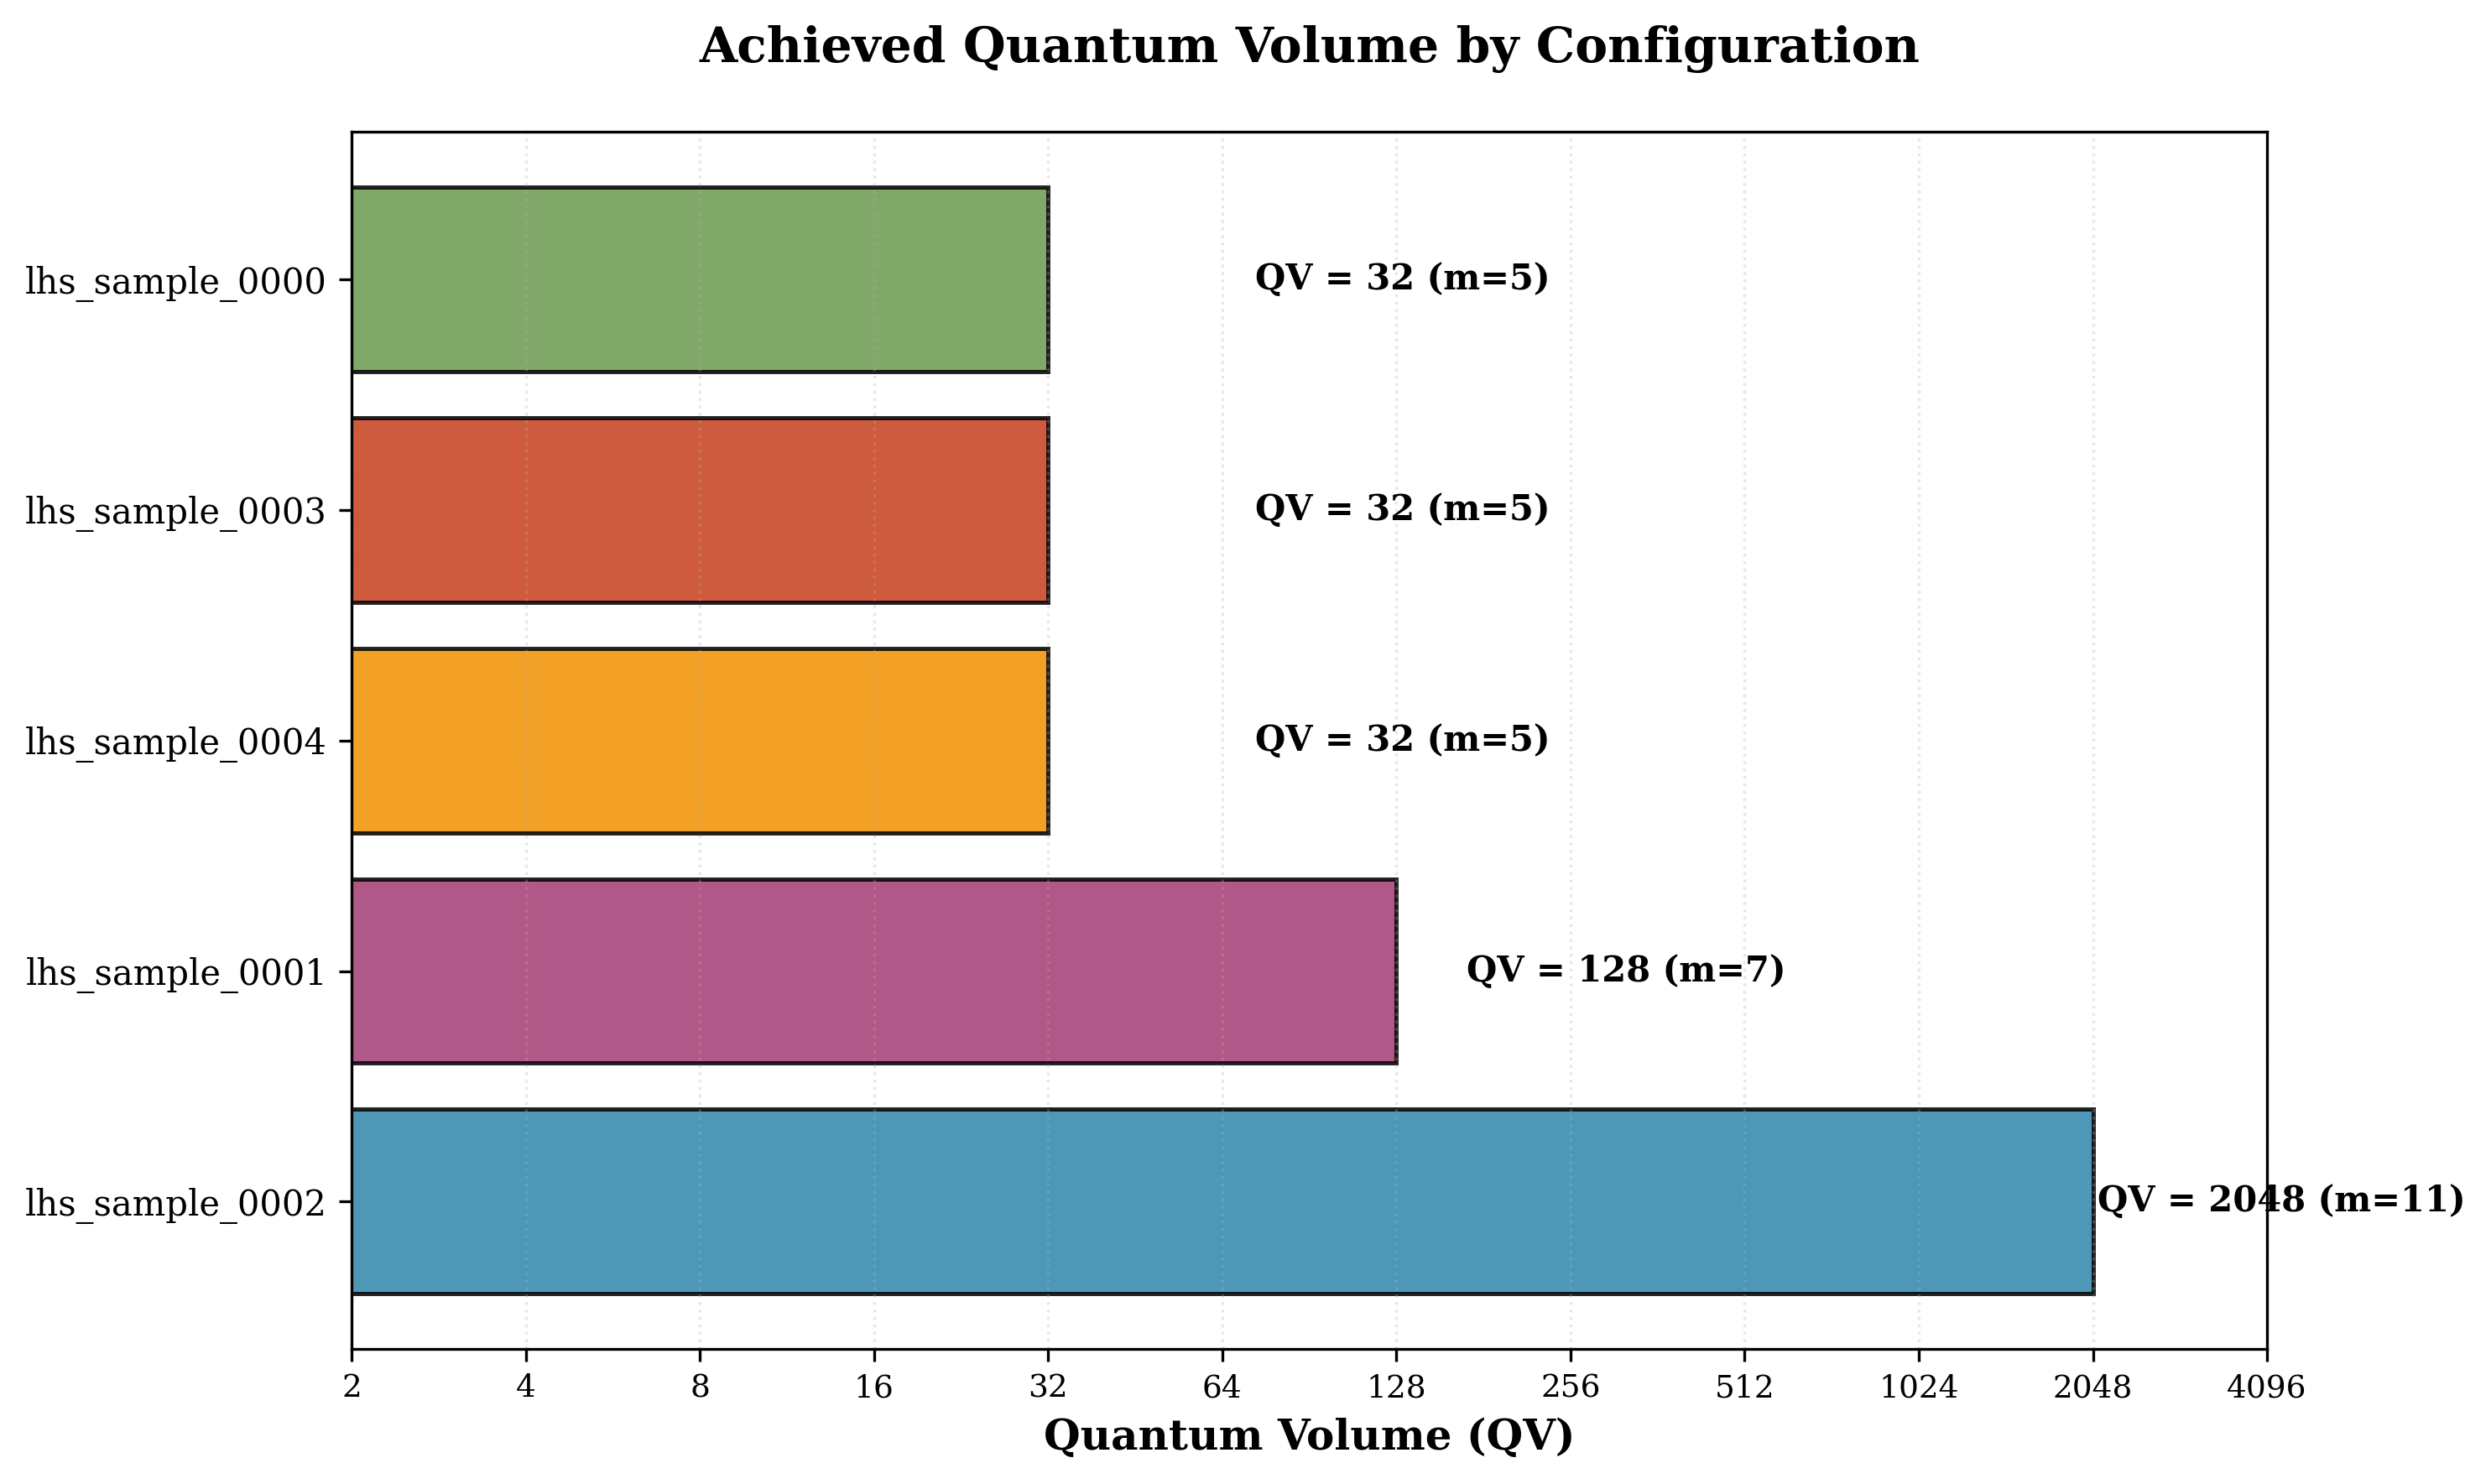
\includegraphics[width=0.85\linewidth]{plots/overview/achieved_qv_comparison.png}
  \caption{Achieved QV across LHS configurations (higher is better).}
  \label{fig:qv-overview}
\end{figure}

\begin{figure}[!htb]
  \centering
  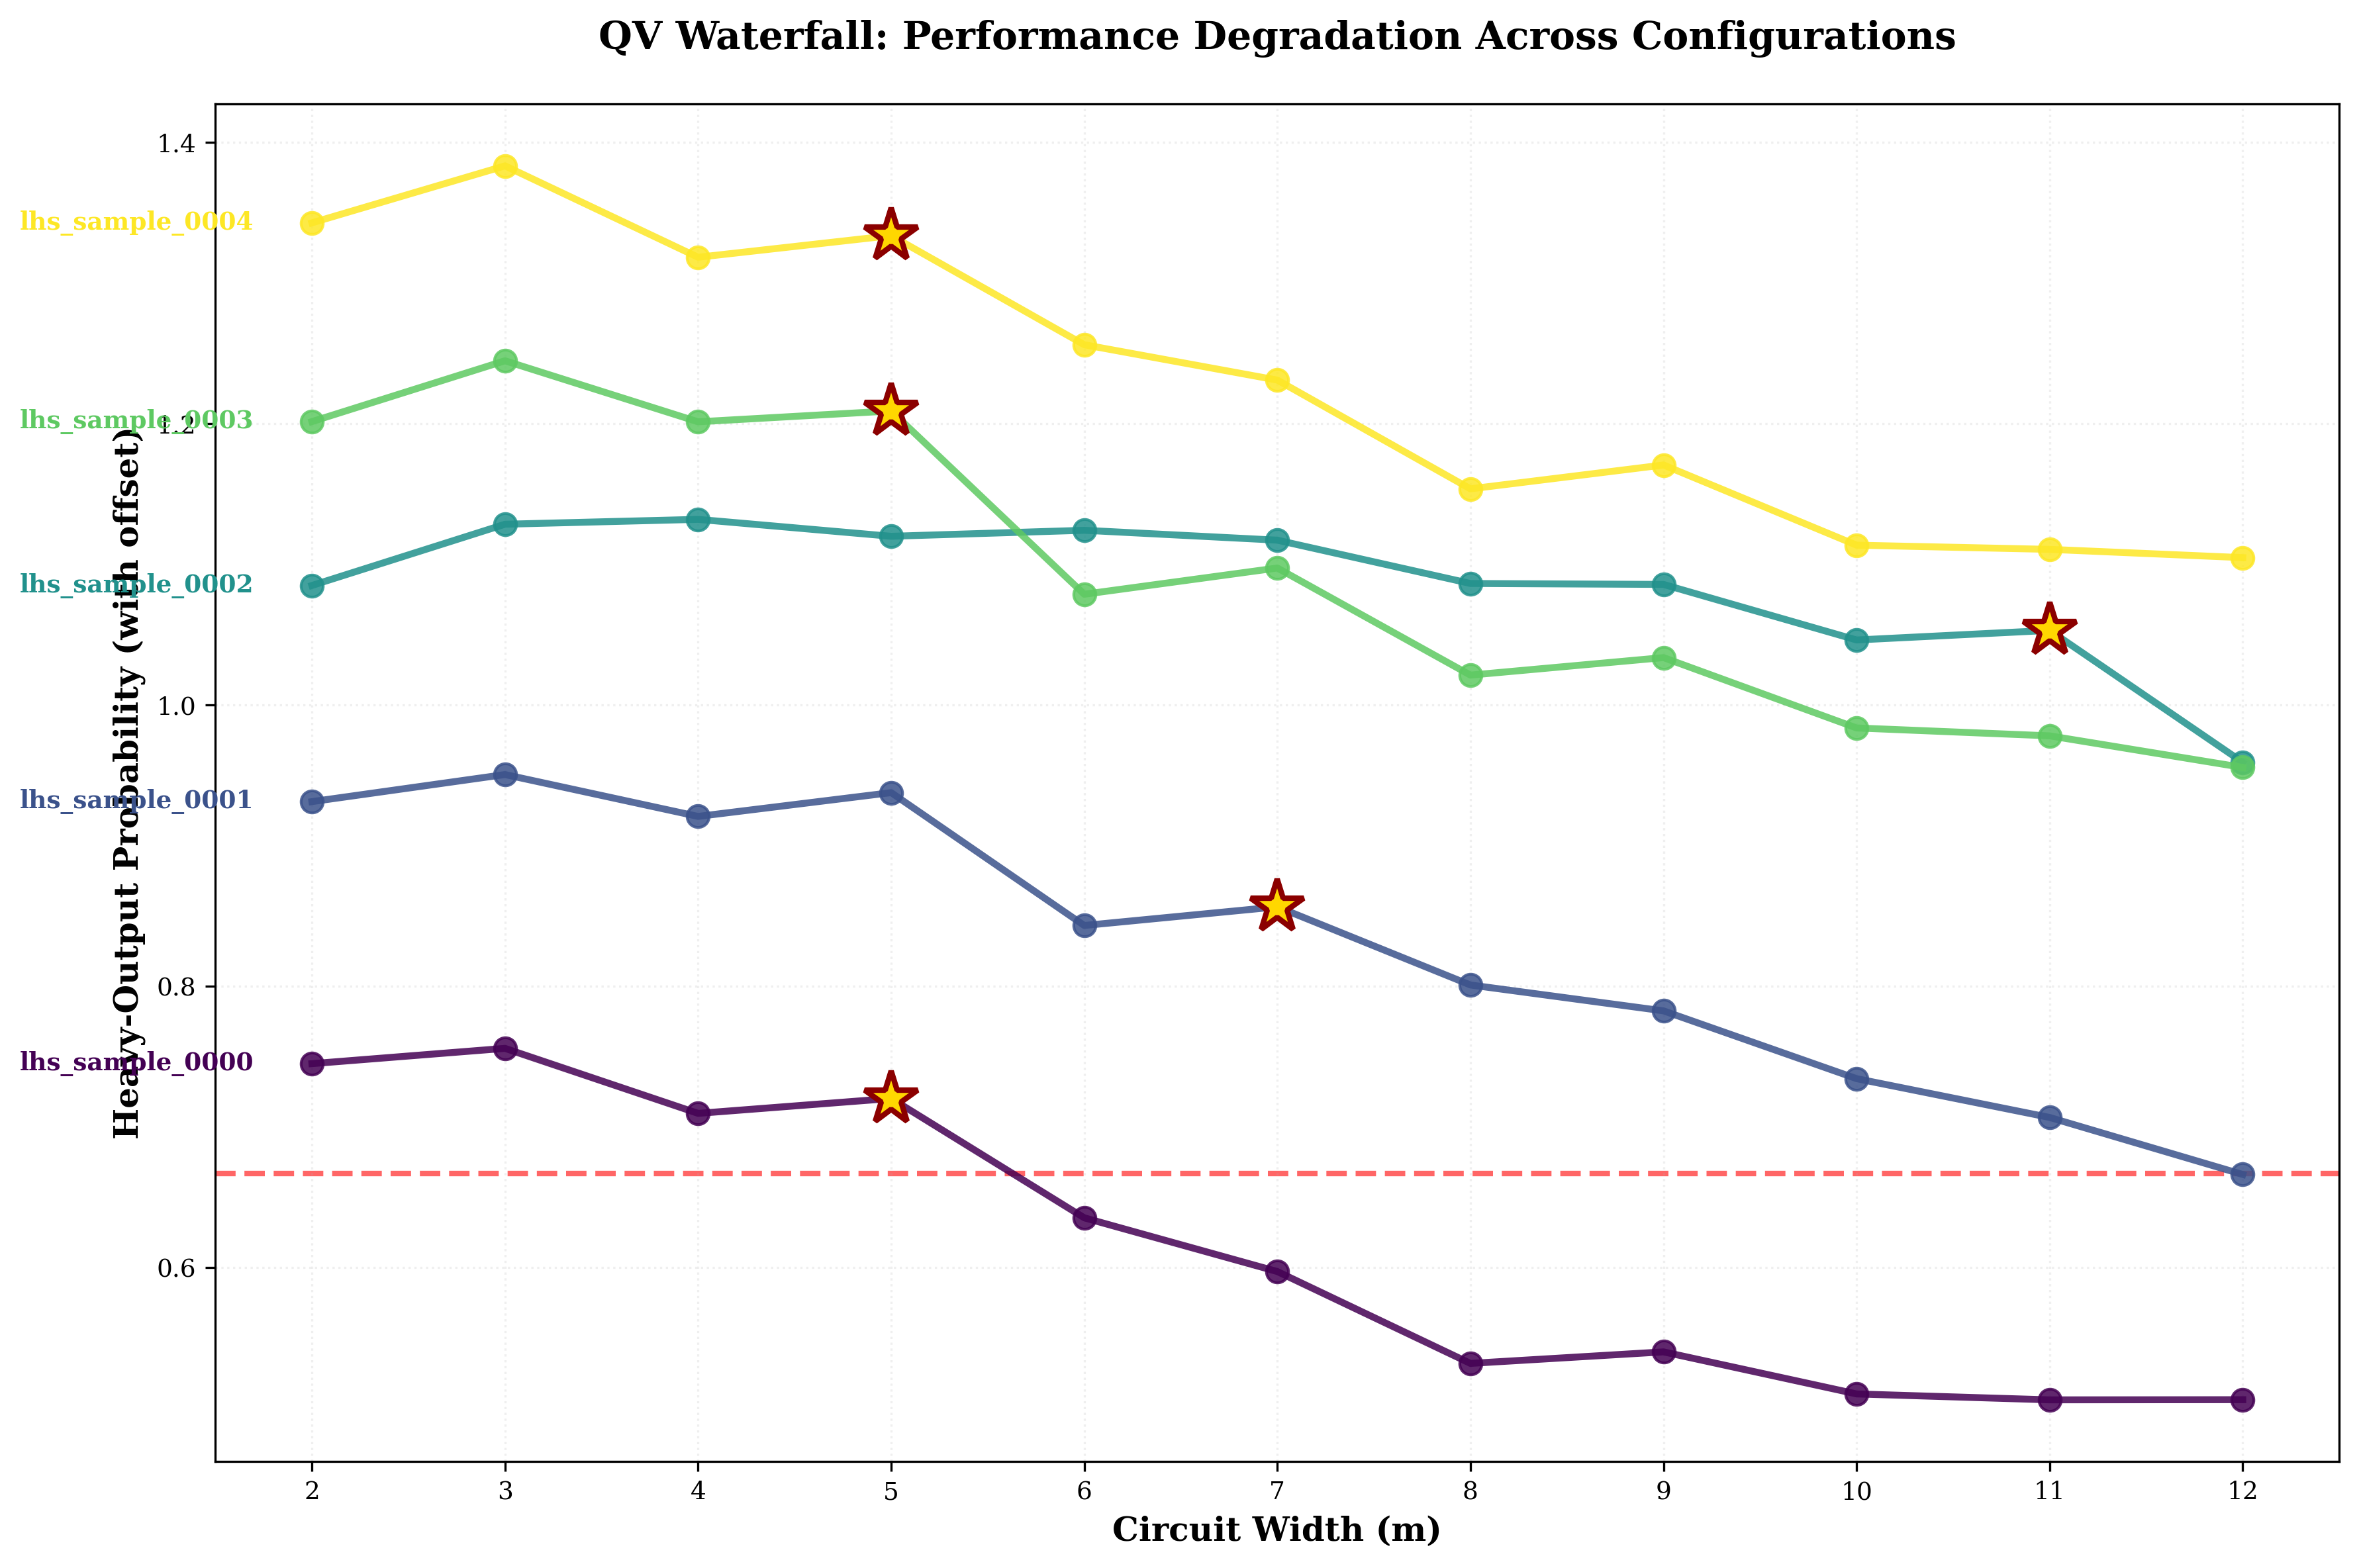
\includegraphics[width=0.85\linewidth]{plots/overview/qv_waterfall.png}
  \caption{QV waterfall by width $m$: heavy-output probability mean and 95\% CI vs threshold.}
  \label{fig:qv-waterfall}
\end{figure}

\subsection{Why lhs\_sample\_0002 achieved a higher QV}
Configuration \texttt{lhs\_sample\_0002} achieved $m^*=11$ ($\mathrm{QV}=2048$), substantially exceeding the other draws. The primary contributors are:
\begin{itemize}
  \item Two-qubit fidelity near the top of the sampled range: $F_2\approx0.99696$ gives $p_{2\mathrm{Q}}=\tfrac{4}{3}(1-F_2)\approx4.06\times10^{-3}$, an order of magnitude lower error than configurations with $F_2\approx0.93$--$0.96$.
  \item Long dephasing times: $T_2\approx2.5$\,ms and $T_2^*\approx16.8$\,$\mu$s reduce both Markovian phase damping during gates and quasi-static detuning per circuit; compare to $T_2^*\lesssim 6$\,$\mu$s in several other samples.
  \item Low measurement error: $P(0\mid1)\approx2.1\times10^{-3}$, which helps preserve HOP at larger widths where SPAM becomes increasingly consequential.
  \item Moderately low residual crosstalk: control crosstalk fraction $\approx1.22\%$ and ZZ-coupling $\sim10$\,kHz (lower than some samples with $\sim25$--$34$\,kHz), limiting coherent error accumulation through the deep, square QV circuits.
\end{itemize}
In combination, these factors keep the mean HOP and its lower 95\% CI above $2/3$ up to $m=11$. By contrast, configurations with lower $F_2$ (e.g., $F_2\approx0.93$) exhibit $p_{2\mathrm{Q}}\approx9.0\times10^{-2}$, leading to early failure at $m\approx5$ even when single-qubit fidelities are high.

\subsection{Connection to cited literature}
The sampled ranges for $F_1$, $F_2$, $T_1$, $T_2$, $T_2^*$, gate times, crosstalk, and SPAM are drawn from recent Si/SiGe spin-qubit reports (see main text references \cite{ref1,ref2,ref4,ref5,ref6,ref9,ref10,ref11}). The mapping from these physical metrics to quantum channels and coherent terms follows the conversion formulas listed above and is consistent with the simulator's unified, constrained error model.

\subsection{Reproducibility notes}
All widths used $N=100$ circuits and 5,000 shots per circuit with fixed RNG seeds per configuration. Backend was statevector with noisy channels applied as described. The JSON files \texttt{campaign\_manifest.json} and \texttt{campaign\_results.json}, together with the YAMLs in \texttt{latex/configs/}, capture the exact parameter draws and outcomes.
